% Analizės modelio dokumentas (2 laboratorinis darbas).
% Kompiliuoti pdfLaTeX iš saugyklos šaknies; visi keliai – nuo šaknies.
% Kiekviena dalis įterpiama komanda \dalis{failas}{pavadinimas}{atsakingas}:
% kol failo nėra, vietoje jo rodoma pavadinta tuščia dalis. Jei savo failą
% padėjote kitu keliu, pataisykite kelią žemiau.
\documentclass[a4paper]{article}
\usepackage[margin=2.5cm]{geometry}
\usepackage{graphicx}
\usepackage[utf8]{inputenc}
\usepackage{lmodern}
\usepackage[T1]{fontenc}
\usepackage[provide=*]{babel}
\usepackage{array}
\usepackage{tabularx}
\usepackage{booktabs}
\usepackage{longtable}
\usepackage{makecell}
\usepackage{float}
\usepackage{pdflscape}
\usepackage{enumitem}
\usepackage{needspace}
\usepackage{caption}
\usepackage{tikz}
\usetikzlibrary{arrows.meta,positioning,calc,shapes.geometric,shapes.multipart}
\usepackage[hidelinks]{hyperref}
% babel lt: „1 lentelė“, „1 pav.“; lentelės pavadinimas virš lentelės, paveikslo – po paveikslu
\captionsetup[table]{labelsep=period}
\captionsetup[figure]{labelsep=space}

\babelprovide[main, import]{lithuanian}

% \dalis{failas}{poskyrio pavadinimas}{atsakingas}
\newcommand{\dalis}[3]{%
  \IfFileExists{#1}{\input{#1}}{\subsection{#2}\textit{[Rengia #3.]}}}

\begin{document}

\begin{titlepage}
    \centering

    {\Large \textbf{Vilniaus Universitetas}}\\[0.2cm]
    {\small Matematikos ir informatikos fakultetas}\\[0.1cm]
    {\small Informatikos katedra}\\[4cm]

    {\huge \textbf{Analizės modelis}}\\[4cm]

    \begin{raggedleft}
    \begin{minipage}{0.55\textwidth}
        \textbf{Atliko:}\\
        Tomas Baublys, Tadas Plančiūnas, Goda Gutparakytė, Marijus Plančiūnas, Ugnė Skučaitė\\[0.8cm]
    \end{minipage}
    \end{raggedleft}

    \vfill

    Vilnius \\ \the\year

\end{titlepage}

\pagebreak

\tableofcontents
\pagebreak

\section{Struktūrinė analizė}\label{sec:strukturine}
\dalis{Struktūrinė analizė/ER diagrama/er_modelis.tex}{Esybių ir ryšių diagrama}{Tomas}
\dalis{Struktūrinė analizė/Duomenų srautai ir gyvavimo ciklai/duomenu_srautu_diagramos_LT.tex}{Duomenų srautų diagramos}{Marijus}
\dalis{Struktūrinė analizė/Duomenų srautai ir gyvavimo ciklai/esybiu_gyvavimo_ciklai_LT.tex}{Esybių gyvavimo ciklai}{Marijus}

\section{Objektinė analizė}\label{sec:objektine}
\dalis{OOA analizė/Analizės klasių diagrama/klasiu_diagrama_LT.tex}{Analizės klasių diagrama}{Tomas}
\dalis{OOA analizė/Panaudojimo atvejų analizė/panaudojimo_atveju_analize_LT.tex}{Panaudojimo atvejų analizė}{Tadas}
\begin{figure}[H]
    \centering
    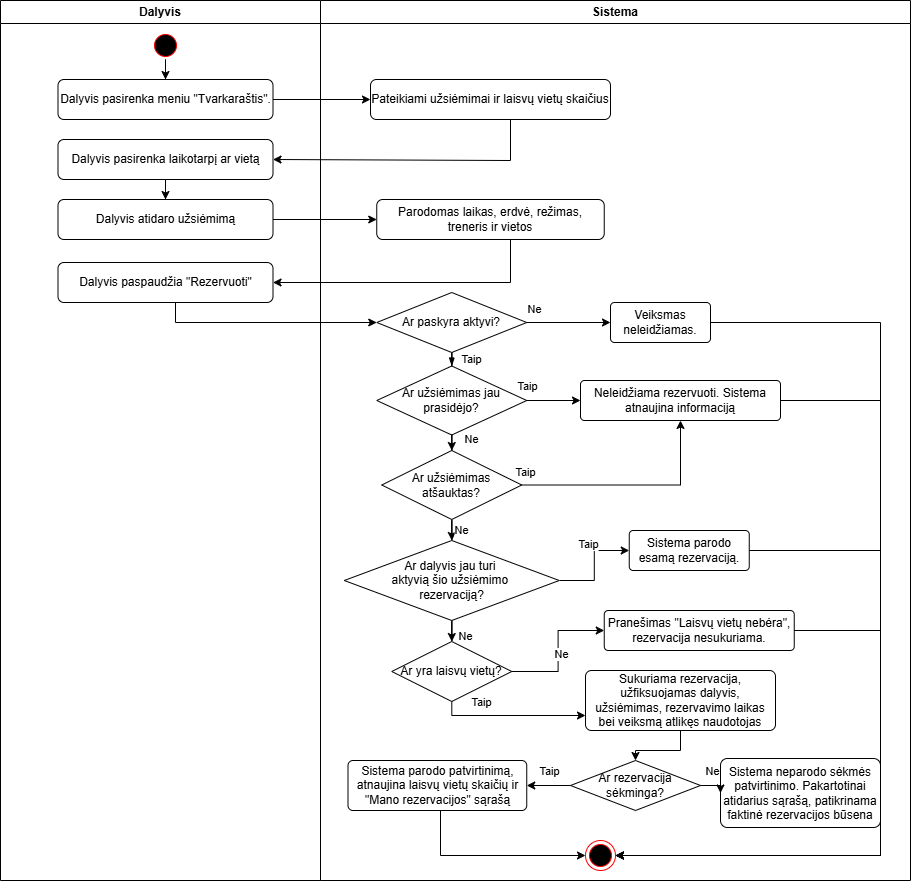
\includegraphics[width=1\linewidth]{OOA analizė/Veiklos diagrama/veiklos diagrama.png}
    \caption{,,PA-09. Rezervuoti vietą užsiėmime'' veiklos diagrama}
    \label{fig:veiklosDiagrama}
\end{figure}

% 3 skyrius „Reikalavimų atsekamumas“ (lentelę sudeda Marijus Plančiūnas).
% Kiekvienas pildo savo stulpelį: ER esybė ir analizės klasė – Tomas,
% DFD procesas – Marijus, panaudojimo atvejis – Tadas. Reikalavimų ID (FR-01, …)
% ir trumpi aprašai – iš Godos Reikalavimų analizės dokumento.

\section{Reikalavimų atsekamumas}\label{sec:analizes-atsekamumas}

Lentelėje kiekvienas funkcinis reikalavimas susietas su jį atspindinčiais
analizės modelio elementais: ER esybėmis (\ref{sec:strukturine}~skyrius),
DFD procesais, analizės klasėmis ir panaudojimo atvejais
(\ref{sec:objektine}~skyrius). Reikalavimų identifikatoriai paimti iš
Reikalavimų analizės dokumento. Nefunkciniai reikalavimai įtraukti tik tie,
kuriuos atspindi kuris nors modelio elementas.

\begingroup
\small
\begin{longtable}{@{}>{\raggedright\arraybackslash}p{1.2cm}>{\raggedright\arraybackslash}p{3.0cm}>{\raggedright\arraybackslash}p{2.5cm}>{\raggedright\arraybackslash}p{1.8cm}>
{\raggedright\arraybackslash}p{3.7cm}>{\raggedright\arraybackslash}p{1.8cm}@{}}
\caption{Reikalavimų ir analizės modelio elementų atsekamumas}\label{tab:analizes-atsekamumas}\\
\toprule
\textbf{ID} & \textbf{Reikalavimas} & \textbf{ER esybė} & \textbf{DFD procesas} & \textbf{Analizės klasė} & \textbf{PA} \\
\midrule
\endfirsthead
\toprule
\textbf{ID} & \textbf{Reikalavimas} & \textbf{ER esybė} & \textbf{DFD procesas} & \textbf{Analizės klasė} & \textbf{PA} \\
\midrule
\endhead
\midrule
\multicolumn{6}{@{}l}{\textit{Funkciniai reikalavimai}} \\
\midrule
FR-01 & Dalyvio registracija sistemoje & Naudotojo paskyra, Dalyvio profilis & 1 & NaudotojoPaskyra, DalyvioProfilis & PA-01 \\
FR-02 & Naudotojo autorizacija (prisijungimas) & Naudotojo paskyra & 1 & NaudotojoPaskyra & PA-01 \\
FR-03 & Užmiršto slaptažodžio atkūrimas & Naudotojo paskyra & 1 & NaudotojoPaskyra & PA-01 \\
FR-04 & Naudotojo asmeninio profilio peržiūra ir redagavimas & Naudotojo paskyra, Dalyvio profilis, Trenerio profilis & 1 & NaudotojoPaskyra, DalyvioProfilis, TrenerioProfilis & PA-01 \\
FR-05 & Vaidmenimis pagrįsta prieigos kontrolė (RBAC) & Naudotojo paskyra & 1 (taikoma ir 4.6, 5, 7) & NaudotojoPaskyra & PA-01, PA-02 \\
FR-06 & Naudotojų paskyrų sukūrimas ir redagavimas administratoriaus sąsajoje & Naudotojo paskyra & 1 & NaudotojoPaskyra & PA-02 \\
FR-07 & Paskyros deaktyvavimas & Naudotojo paskyra, Rezervacija & 1 & NaudotojoPaskyra, Rezervacija & PA-02 \\
FR-08 & Naudotojų sąrašo ir detalių peržiūra & Naudotojo paskyra, Dalyvio profilis & 1 & NaudotojoPaskyra, DalyvioProfilis & PA-02 \\
FR-09 & Sporto erdvių registras & Sporto erdvė, Erdvės vaizdo ir garso profilis & 1 & SportoErdvė, ErdvėsVaizdoIrGarsoProfilis & PA-03 \\
FR-10 & Techninės įrangos valdymo ir nustatymų registras & Įrenginys, Vaizdo / Garso įrenginio nustatymai & 1 & Įrenginys, VaizdoĮrenginioNustatymai, GarsoĮrenginioNustatymai & PA-03 \\
FR-11 & Mokomosios vaizdo ir garso medžiagos valdymas & Mokomoji medžiaga & 2 & MokomojiMedžiaga & PA-04 \\
FR-12 & Pratimų katalogo valdymas ir paieška & Pratimas, Mokomoji medžiaga & 2 & Pratimas, MokomojiMedžiaga & PA-04 \\
FR-13 & Užsiėmimo programos kūrimas ir peržiūra & Užsiėmimo programa, Programos versija, Programos etapas & 2 & UžsiėmimoPrograma, ProgramosVersija, ProgramosEtapas & PA-05 \\
FR-14 & Programos etapų valdymas & Programos etapas, Etapo pratimas, Pratimas, Mokomoji medžiaga & 2 & ProgramosEtapas, Pratimas, MokomojiMedžiaga & PA-05 \\
FR-15 & Programų versijavimas, archyvavimas ir istorija & Užsiėmimo programa, Programos versija, Trenerio profilis & 2 & UžsiėmimoPrograma, ProgramosVersija, TrenerioProfilis & PA-05 \\
FR-16 & Grupinių ir individualių užsiėmimų planavimas & Užsiėmimas, Užsiėmimo nustatymai, Sporto erdvė & 3 & Užsiėmimas, UžsiėmimoNustatymai, SportoErdvė & PA-06 \\
FR-17 & Virtualaus trenerio užsiėmimų planavimas & Užsiėmimas, Sporto erdvė, Užsiėmimo programa & 3 & Užsiėmimas, SportoErdvė, UžsiėmimoPrograma & PA-07 \\
FR-18 & Užsiėmimo duomenų keitimas ir informavimas & Užsiėmimas, Užsiėmimo nustatymai, Rezervacija & 3 & Užsiėmimas, UžsiėmimoNustatymai, Rezervacija & PA-08 \\
FR-19 & Užsiėmimo atšaukimas ir rezervacijų anuliavimas & Užsiėmimas, Rezervacija & 3 & Užsiėmimas, Rezervacija & PA-08 \\
FR-20 & Užsiėmimo eigos paleidimas ir užbaigimas & Užsiėmimas, Vykdymo žurnalas & 6.2, 6.6 & Užsiėmimas, VykdymoŽurnalas & PA-15 \\
FR-21 & Užsiėmimo eigos pristabdymas ir tęsimas & Užsiėmimas, Vykdymo žurnalas & 6.2 & Užsiėmimas, VykdymoŽurnalas & PA-15 \\
FR-22 & Etapų praleidimas ir eiliškumo keitimas realiuoju laiku & Užsiėmimas, Programos etapas & 6.2 & Užsiėmimas, ProgramosEtapas & PA-15 \\
FR-23 & Etapo trukmės koregavimas vykdymo metu & Užsiėmimas, Programos etapas & 6.2 & Užsiėmimas, ProgramosEtapas & PA-15 \\
FR-24 & Valdymo pulto būsenos atvaizdavimas & Užsiėmimas, Vykdymo žurnalas & 6.2, 6.3 & Užsiėmimas, VykdymoŽurnalas & PA-15 \\
FR-25 & Virtualaus trenerio autonominis vykdymas & Užsiėmimas, Programos versija & 6.1, 6.2, 6.3 & Užsiėmimas, ProgramosVersija & PA-07, PA-15 \\
FR-26 & Tvarkaraščio ir laisvų vietų peržiūra & Užsiėmimas, Rezervacija & 4.1 & Užsiėmimas, Rezervacija & PA-09 \\
FR-27 & Vietos rezervavimas užsiėmime & Rezervacija, Užsiėmimas, Naudotojo paskyra & 4.2 & Rezervacija, Užsiėmimas & PA-09 \\
FR-28 & Rezervacijos atšaukimas dalyvio iniciatyva & Rezervacija & 4.3 & Rezervacija & PA-10 \\
FR-29 & Asmeninės rezervacijų istorijos peržiūra & Rezervacija, Naudotojo paskyra & 4.1, 4.8 & Rezervacija & PA-09 \\
FR-30 & Dalyvio priskyrimas prie užsiėmimo rankiniu būdu & Rezervacija, Užsiėmimas, Dalyvio profilis & 4.4 & Rezervacija, Užsiėmimas, DalyvioProfilis & PA-11 \\
FR-31 & Dalyvio pašalinimas iš užsiėmimo sąrašo & Rezervacija, Užsiėmimas & 4.4 & Rezervacija, Užsiėmimas & PA-11 \\
FR-32 & Užsiėmimo dalyvių sąrašo ir kortelių peržiūra & Rezervacija, Užsiėmimas, Dalyvio profilis & 4.6 & Rezervacija, Užsiėmimas, DalyvioProfilis & PA-11 \\
FR-33 & Faktinio lankomumo žymėjimas ir taisymas & Lankomumo įrašas, Rezervacija & 4.5 & LankomumoĮrašas, Rezervacija & PA-12 \\
FR-34 & Lankomumo istorijos peržiūra & Lankomumo įrašas, Rezervacija & 4.5, 4.10 & LankomumoĮrašas, Rezervacija & PA-12 \\
FR-35 & Automatiniai priminimai apie užsiėmimą & Rezervacija, Užsiėmimas, Naudotojo paskyra & 4.7 & Rezervacija, Užsiėmimas & PA-18 \\
FR-36 & Dalyvio įvertinimo įrašymas & Įvertinimas, Dalyvio profilis & 5 & Įvertinimas, DalyvioProfilis & PA-13 \\
FR-37 & Asmeninės programos sudarymas ir rekomendacijos & Įvertinimas, Asmeninė programa, Pasiruošimo rekomendacija & 5 & Įvertinimas, AsmeninėPrograma, PasirengimoRekomendacija & PA-13 \\
FR-38 & Namų užduočių priskyrimas & Namų užduotis, Pratimas & 5 & NamųUžduotis, Pratimas & PA-14 \\
FR-39 & Nuotolinis asmeninės programos ir užduočių redagavimas & Asmeninė programa, Namų užduotis & 5 & AsmeninėPrograma, NamųUžduotis & PA-13, PA-14 \\
FR-40 & Asmeninės programos archyvavimas ir užduočių šalinimas & Asmeninė programa, Namų užduotis & 5 & AsmeninėPrograma, NamųUžduotis & PA-13, PA-14 \\
FR-41 & Asmeninių programų sąrašo ir detalių peržiūra & Asmeninė programa, Namų užduotis & 5 & AsmeninėPrograma, NamųUžduotis & PA-13, PA-14 \\
FR-42 & Užsiėmimo etapo vaizdo demonstravimas ekrane & Užsiėmimas, Programos etapas, Mokomoji medžiaga & 6.3, 6.4 & Užsiėmimas, ProgramosEtapas, MokomojiMedžiaga & PA-15 \\
FR-43 & Autonominis grotuvo veikimas nutrūkus ryšiui & Užsiėmimas, Vykdymo žurnalas & 6.3, 6.6 & Užsiėmimas, VykdymoŽurnalas & PA-16 \\
FR-44 & Garso instrukcijų ir trenerio balso transliacija & Mokomoji medžiaga, Įrenginys, Garso įrenginio nustatymai & 6.5 & MokomojiMedžiaga, Įrenginys, GarsoĮrenginioNustatymai & PA-15 \\
FR-45 & Užsiėmimų eigos istorijos saugojimas & Užsiėmimas, Vykdymo žurnalas & 6.6, 7 & Užsiėmimas, VykdymoŽurnalas & PA-17 \\
FR-46 & Lankomumo ir užimtumo ataskaitų generavimas & Užsiėmimas, Rezervacija, Lankomumo įrašas, Sporto erdvė & 7 & Užsiėmimas, Rezervacija, LankomumoĮrašas, SportoErdvė & PA-17 \\
\midrule
\multicolumn{6}{@{}l}{\textit{Nefunkciniai reikalavimai, atspindėti modelio elementuose}} \\
\midrule
NFR-07, NFR-08 & Asmens duomenų saugojimo terminai, kopija ir anonimizavimas & Naudotojo paskyra, Dalyvio profilis, Rezervacija, Lankomumo įrašas & 1, 4 & NaudotojoPaskyra, DalyvioProfilis, Rezervacija, LankomumoĮrašas & PA-01, PA-02 \\
NFR-09, NFR-24 & Prieiga prie jautrių profilio duomenų ir trenerio / dalyvio prieigos ribos & Dalyvio profilis, Rezervacija, Užsiėmimas & 4.6, 5 & DalyvioProfilis, Rezervacija, Užsiėmimas & PA-11, PA-12, PA-14 \\
NFR-10 & Bazinės versijos apimtis – vienas centras & Sporto erdvė, Įrenginys & 1 & SportoErdvė, Įrenginys & PA-03 \\
NFR-13 & Vaizdo turinio raiška (Full HD) & Mokomoji medžiaga & 2 & MokomojiMedžiaga & PA-04 \\
NFR-17, NFR-18 & Užsiėmimo tęstinumas sutrikus ryšiui; turinio atsisiuntimas į grotuvą & Užsiėmimas, Vykdymo žurnalas & 6.1, 6.3, 6.6 & Užsiėmimas, VykdymoŽurnalas & PA-15, PA-16 \\
NFR-23, NFR-27 & Priminimų siuntimo laikas, unikalumas ir pakartojimas & Rezervacija, Užsiėmimas & 4.7 & Rezervacija & PA-18 \\
NFR-25 & Paskutinės laisvos vietos rezervavimas lygiagrečiai & Rezervacija, Užsiėmimas & 4.2, 4.4 & Rezervacija, Užsiėmimas & PA-09, PA-11 \\
NFR-26 & Lankomumo ir rezervacijų pakeitimų atsekamumas & Rezervacija, Lankomumo įrašas & 4.3, 4.4, 4.5 & Rezervacija, LankomumoĮrašas & PA-10, PA-11, PA-12 \\
NFR-42, NFR-43 & Istorijos saugojimo trukmė; rezervacijų ir lankomumo įrašų išlikimas & Užsiėmimas, Rezervacija, Lankomumo įrašas & 3, 4, 7 & Užsiėmimas, Rezervacija, LankomumoĮrašas & PA-08, PA-12, PA-17 \\
NFR-30 & Prisitaikanti sąsaja telefonui, planšetei ir kompiuteriui & Asmeninė programa & 5 & AsmeninėPrograma & PA-13, PA-14 \\
\bottomrule
\end{longtable}
\endgroup

\end{document}
